\documentclass[10pt,a4paper,twocolumn]{article}
\usepackage[a4paper,top=20mm,bottom=22mm,left=17mm,right=17mm,columnsep=7mm]{geometry}
\usepackage{fontspec}
\usepackage{amsmath,amsthm}
\usepackage{unicode-math}
\setmainfont{Liberation Serif}
\setsansfont{Liberation Sans}
\setmonofont{DejaVu Sans Mono}[Scale=0.78]
\setmathfont{Latin Modern Math}
\usepackage{polyglossia}
\setdefaultlanguage{russian}
\setotherlanguage{english}
\newfontfamily\cyrillicfont{Liberation Serif}
\newfontfamily\cyrillicfontsf{Liberation Sans}
\newfontfamily\cyrillicfonttt{DejaVu Sans Mono}[Scale=0.78]
\usepackage{microtype}
\usepackage{graphicx}
\usepackage{booktabs,tabularx,array}
\usepackage[font=small,labelfont=bf,labelsep=period]{caption}
\usepackage{enumitem}
\setlist{nosep,leftmargin=1.4em}
\usepackage{titlesec}
\titleformat{\section}{\normalfont\large\bfseries}{\thesection.}{0.5em}{}
\titleformat{\subsection}{\normalfont\normalsize\bfseries}{\thesubsection.}{0.5em}{}
\titlespacing*{\section}{0pt}{1.6ex plus .5ex}{0.8ex}
\titlespacing*{\subsection}{0pt}{1.2ex plus .4ex}{0.5ex}
\usepackage{fancyvrb}
\usepackage{xurl}
\usepackage[hidelinks]{hyperref}
\urlstyle{tt}
\hypersetup{pdftitle={Сарафанное радио: когда сеть обгоняет прямой канал},pdfauthor={Валентин Алексеев},pdfsubject={Grapevine versus the official channel},pdfkeywords={rumour, information theory, covering number, cheap talk, disclosure, Lean}}
\usepackage{fancyhdr}
\pagestyle{fancy}
\fancyhf{}
\fancyhead[L]{\footnotesize\itshape Сарафанное радио: когда сеть обгоняет прямой канал}
\fancyhead[R]{\footnotesize\thepage}
\renewcommand{\headrulewidth}{0.3pt}

\theoremstyle{plain}
\newenvironment{stmt}[1]{\par\smallskip\noindent\textbf{#1.}\ \itshape}{\par\smallskip}
\newenvironment{dfn}[1]{\par\smallskip\noindent\textbf{#1.}\ }{\par\smallskip}
\renewcommand{\proofname}{Доказательство}
\newcommand{\lean}[1]{{\footnotesize\nolinkurl{#1}}}
\newcommand{\leanref}[1]{\par\noindent{\footnotesize Lean: #1}\par\smallskip}
\newcommand{\txt}[1]{\text{#1}}
\setlength{\parskip}{0pt}
\setlength{\parindent}{1.2em}
\raggedbottom
\renewcommand{\dbltopfraction}{0.85}
\renewcommand{\textfraction}{0.1}
\renewcommand{\topfraction}{0.85}
\setcounter{dbltopnumber}{3}

\begin{document}

\twocolumn[{%
\begin{center}
{\LARGE\bfseries Сарафанное радио: когда сеть\\[2pt] обгоняет прямой канал\par}
\vspace{6pt}
{\large Валентин Алексеев\par}
\vspace{2pt}
{\small 1 ноября 2026 г.\par}
\vspace{10pt}
\begin{minipage}{0.86\textwidth}
\begin{english}
\small
\noindent\textbf{Abstract.}
We formalize the hypothesis that an agent $Z$ can reconstruct a message from fragmentary and partly unreliable network reports faster than it receives the exact message directly from its source $A$. In its universal form the claim is false, by causality and by the data-processing inequality. We prove that in a one-shot model it holds if and only if
$\lceil \log_2 N(\varepsilon) \rceil \le C\,(T-1-d)$, where $N(\varepsilon)$ is the covering number of the receiver's residual uncertainty at error tolerance $\varepsilon$, $C$ the min-cut capacity of the network, $d$ its minimal delay and $T$ the time of direct delivery. When the source does not know what the receiver knows, the exact criterion becomes a colouring condition on a confusability graph, and the price of this ignorance is bounded by $\log_2\big((\Delta+1)/\max_y |M_y|\big)$ bits. We extend the model to gradual disclosure by an authoritative source, showing that decision-first ordering is optimal and that silence carries information; to leakage risk, which scales with the number of independent circles of insiders rather than with the number of people; and to cheap talk, where a conflict of interest $b$ caps credible information at $\log_2 N(b)$ bits per round (Crawford--Sobel). As a consequence we study premature actions taken on rumours: disclosure that fully resolves the decision-relevant question for a group eliminates regretted actions in that group, whereas partial disclosure that leaves it open can increase them. All 91 statements are machine-checked in Lean~4 with Mathlib; Monte Carlo simulations illustrate magnitudes, and six falsifiable predictions are stated.

\smallskip
\noindent\textbf{Keywords:} rumour, information theory, covering number, side information, Witsenhausen, cheap talk, disclosure policy, formal verification, Lean.
\end{english}

\medskip
\noindent\textbf{Аннотация.}
Получатель $Z$ может восстановить сообщение по обрывкам из сети раньше, чем получит его напрямую от источника $A$, тогда и только тогда, когда информации, которой ему не хватает, меньше, чем сеть успевает доставить до прихода прямого сообщения. Мы формализуем эту гипотезу о «сарафанном радио», доказываем необходимое условие и точный критерий, в том числе для случая, когда источник не знает, что известно получателю. Отдельно рассмотрены мозаичный эффект, риск утечки, конфликт интересов, постепенное раскрытие авторитетным источником и практическое следствие — преждевременные действия на слухах. Все 91 утверждение проверены в Lean~4; приводятся симуляции и шесть проверяемых предсказаний.

\smallskip
\noindent\textbf{Ключевые слова:} слухи, теория информации, число покрытия, побочная информация, дешёвые разговоры, политика раскрытия, формальная верификация.
\end{minipage}
\end{center}
\vspace{12pt}
}]

\section{Введение}

Исходная гипотеза: в сети из многих узлов получатель $Z$ восстанавливает сообщение из $A$ по частичным и местами искажённым обрывкам с достаточной точностью быстрее, чем получит точное сообщение напрямую. Это наблюдение знакомо каждому, кто узнавал о реорганизации из слухов за недели до официального объявления.

В универсальной форме («всегда быстрее») гипотеза ложна по двум причинам.
\emph{Причинность}: каждый обрывок идёт к $Z$ по какому-то пути, и если прямой канал и есть самый быстрый путь, ни один обрывок не придёт раньше.
\emph{Неравенство обработки данных}: пересказы не содержат о сообщении больше информации, чем само сообщение.

Поэтому правильный вопрос — не «верна ли гипотеза», а «при каких условиях». Интуиция подсказывает три механизма выигрыша, и все три входят в итоговое неравенство:
\begin{enumerate}
\item широкая сеть против узкого прямого канала;
\item знания получателя: ему нужно узнать не всё сообщение, а только то, что отличает его от уже известных вариантов;
\item допустимая ошибка: для решения часто хватает приближённого понимания.
\end{enumerate}

\textbf{Что известно и что добавлено.} Известны граница минимального разреза для потока информации~\cite{ahlswede}, кодирование с искажением~\cite{shannon}, кодирование с побочной информацией~\cite{slepianwolf,wynerziv}, однократная задача с побочной информацией и хроматические числа~\cite{witsenhausen}, модель Кроуфорда–Собела~\cite{crawfordsobel}, схема Шамира~\cite{shamir}. В работе добавлены: сравнение сети с прямым каналом во времени и точные однократные критерии выигрыша; двусторонняя оценка цены незнания источника; обратная задача — оценка пропускной способности неформальных каналов по наблюдению; оценка риска утечки через число независимых кругов посвящённых; постепенное раскрытие и его следствие для преждевременных действий; проверяемые предсказания; машинная проверка всех доказательств.

\section{Модель и обозначения}

Время дискретно, информация измеряется в битах.

\begin{center}
\small
\begin{tabularx}{\columnwidth}{@{}lX@{}}
\toprule
$A$, $Z$ & источник и получатель \\
$M$ & сообщения, которые $Z$ до передачи считает возможными \\
$\rho(m,\hat m)$ & мера ошибки между $m$ и восстановленным $\hat m$ \\
$\varepsilon$ & допустимая ошибка \\
$V(\varepsilon)$ & наибольшее число сообщений в шаре ошибки \\
$d$ & минимальная задержка сети \\
$C$ & пропускная способность минимального разреза, бит/такт \\
$T$ & момент прямой доставки точного сообщения \\
\bottomrule
\end{tabularx}
\end{center}

Шар ошибки и его размер:
\[
B_\varepsilon(c) = \{x \in M : \rho(c,x) \le \varepsilon\},\qquad V(\varepsilon) = \max_c |B_\varepsilon(c)|.
\]

\begin{dfn}{Предположение о сети}
К моменту $\tau$ в $Z$ попадает не больше $b(\tau) \le C\cdot\max(0,\tau-d)$ бит. По теореме Альсведе–Кая–Ли–Янга~\cite{ahlswede} скорость $C$ достижима, если узлы кодируют данные.
\end{dfn}

\begin{dfn}{Определение 1}
$Z$ восстанавливает сообщение с ошибкой $\varepsilon$ по $b$ битам, если существуют $\mathrm{enc}\colon M\to\{0,1\}^b$ и $\mathrm{dec}\colon\{0,1\}^b\to M$ такие, что $\rho(\mathrm{dec}(\mathrm{enc}(m)),m)\le\varepsilon$ для \emph{каждого} $m$. Кодировщик и декодер произвольны, поэтому отрицательные результаты верны при любой стратегии участников.
\end{dfn}

\begin{dfn}{Определение 2}
Сеть выигрывает, если найдётся $\tau<T$, к которому $Z$ восстанавливает сообщение с ошибкой $\varepsilon$ по $b(\tau)$ битам.
\end{dfn}

\section{Теорема 1: необходимое условие}

\begin{stmt}{Лемма 1 (о покрытии)}
Если $Z$ восстанавливает любое сообщение из $M$ с ошибкой не больше $\varepsilon$ по $b$ битам, то $|M| \le 2^b\, V(\varepsilon)$.
\end{stmt}
\begin{proof}
Каждой из $2^b$ строк декодер ставит в соответствие ответ $\mathrm{dec}(w)$. Сообщение $m$ лежит в шаре $B_\varepsilon(\mathrm{dec}(\mathrm{enc}(m)))$, поэтому
\[
|M| \le \sum_{w} |B_\varepsilon(\mathrm{dec}(w))| \le 2^b\, V(\varepsilon). \qedhere
\]
\end{proof}

\begin{stmt}{Теорема 1}
Если сеть выигрывает при допустимой ошибке $\varepsilon$, то
\[
\log_2|M| - \log_2 V(\varepsilon) \le C\,(T-1-d).
\]
\end{stmt}
\begin{proof}
Пусть $\tau\le T-1$. Тогда $b(\tau)\le C(\tau-d)\le C(T-1-d)$, и по лемме~1 $|M|\le 2^{C(T-1-d)}V(\varepsilon)$.
\end{proof}
\leanref{\lean{covering_bound}, \lean{rumour_general}, \lean{rumour_general_loses}.}

Левая часть зависит только от получателя: чем больше $Z$ знает (меньше $|M|$) и чем грубее ему достаточно знать (больше $V(\varepsilon)$), тем она меньше. Правая часть зависит только от сети и прямого канала.

\textit{Пример.} $Z$ ждёт цену сделки, одно из 1024 значений, и ему хватает точности до восьми соседних ($V=8$): нужно 7 бит. При $d=3$ и $C=2$ сеть может выиграть, если $T=10$ ($2\cdot6=12\ge7$), и не может, если $T=6$ ($2\cdot2=4<7$).

\subsection{Теорема 1$'$: точная версия}

Шары ошибки могут перекрываться, и тогда неравенство $|M|\le 2^bV(\varepsilon)$ выполнено, а $b$ бит всё равно не хватает. Точный ответ даёт \emph{число покрытия} $N(\varepsilon)$ — наименьшее число шаров, покрывающих $M$.

\begin{stmt}{Теорема 1$'$}
Пусть сеть доставляет к моменту $\tau$ ровно $C(\tau-d)$ бит. Тогда
\[
\text{сеть выигрывает} \iff \lceil\log_2 N(\varepsilon)\rceil \le C\,(T-1-d),
\]
причём $|M|/V(\varepsilon)\le N(\varepsilon)\le|M|$.
\end{stmt}
\begin{proof}
Восстановление по $b$ битам равносильно покрытию $M$ шарами с центрами $\mathrm{dec}(w)$: в одну сторону центрами служат ответы декодера, в другую кодировщик передаёт номер ближайшего центра. Покрытие можно дополнить лишними центрами, поэтому оно существует на $2^b$ шарах тогда и только тогда, когда $N(\varepsilon)\le 2^b$.
\end{proof}
\leanref{\lean{Exact.rumour_exact_informed}, \lean{Exact.card_le_coverNum_mul}.}

\section{Теорема 2: источник не знает, что известно $Z$}

В теореме~1 знания $Z$ сужают $M$ «для всех»: неявно считается, что $A$ знает, что известно $Z$. В реальной сети это не так.

\begin{dfn}{Постановка}
$X$ — все сообщения, $Y$ — состояния знаний $Z$; $\mathrm{compat}(x,y)$ означает, что $x$ не противоречит знаниям $y$. Кодировщик видит только $x$, декодер — полученные биты и $y$:
\[
\mathrm{compat}(x,y)\Rightarrow\rho\big(\mathrm{dec}(\mathrm{enc}(x),y),x\big)\le\varepsilon.
\]
Раскраска $c\colon X\to\{0,1\}^b$ \emph{допустима}, если для любых $y$ и цвета $w$ все сообщения цвета $w$, совместимые с $y$, лежат в одном шаре радиуса $\varepsilon$.
\end{dfn}

\begin{stmt}{Теорема 2}
Задача решается $b$ битами тогда и только тогда, когда есть допустимая раскраска в $2^b$ цветов. Если сеть доставляет ровно $C(\tau-d)$ бит, то сеть выигрывает $\iff$ существует допустимая раскраска в $2^{C(T-1-d)}$ цветов.
\end{stmt}
\begin{proof}
($\Rightarrow$) $c=\mathrm{enc}$, центр шара для $(y,w)$ — $\mathrm{dec}(w,y)$. ($\Leftarrow$) $\mathrm{enc}=c$, $\mathrm{dec}(w,y)$ — центр шара для $(y,w)$. Вторая часть следует из монотонности по числу бит.
\end{proof}
\leanref{\lean{SideInfo.solvable_iff}, \lean{SideInfo.rumour_exact}.}

При нулевой ошибке допустимая раскраска — это правильная раскраска графа неразличимости $G$: два сообщения соединены, если при каких-то знаниях $Z$ не может исключить ни одно из них. Минимальное число бит равно $\lceil\log_2\chi(G)\rceil$~\cite{witsenhausen}.

\textit{Пример: цена незнания.} Пять сообщений по кругу; $Z$ знает, что сообщение — $y$ или $y+1 \pmod 5$. Если $A$ знает $y$, хватает 1 бита. Если нет, граф неразличимости — цикл $C_5$, $\chi=3$, и нужно 2 бита.
\leanref{\lean{SideInfo.goodColoring_zero_iff}, \lean{Pentagon.price_of_blindness}.}

\subsection{Двусторонняя оценка цены незнания}

Пусть $M_y$ — сообщения, совместимые со знаниями $y$, а $\Delta$ — наибольшая степень графа неразличимости.

\begin{stmt}{Теорема 2$'$}
Необходимое число бит $b^*$ при нулевой ошибке удовлетворяет
\[
\log_2\max_y|M_y| \;\le\; b^* \;\le\; \lceil\log_2(\Delta+1)\rceil.
\]
\end{stmt}
\begin{proof}
Нижняя граница — лемма~1 для каждого $y$ при $V=1$. Верхняя — жадная раскраска: у очередного сообщения не больше $\Delta$ окрашенных соседей, поэтому из $\Delta+1$ цвета всегда есть свободный.
\end{proof}
\leanref{\lean{Exact.greedy}, \lean{Exact.blind_lower}, \lean{Exact.blind_upper}, \lean{Exact.pentagon_bounds}.}

В пятиугольнике $\max|M_y|=2$ и $\Delta=2$: границы 1 и 2 бита, нужно ровно 2 — верхняя граница достигается.

Для длинной передачи с малой вероятностью ошибки цена незнания исчезает: по теореме Слепяна–Вулфа~\cite{slepianwolf} достаточно $R=H(X\mid Y)$. При $\varepsilon>0$ (постановка Вайнера–Зива~\cite{wynerziv}) небольшая потеря в общем случае остаётся.

\section{Следствия и частные случаи}

\begin{stmt}{Следствие 1 (причинность)}
Если $T\le d$, сеть не выигрывает ни при каком $\varepsilon$, если $|M|>V(\varepsilon)$.
\end{stmt}
\leanref{\lean{causality}, \lean{SideInfo.announce_first}.}

\begin{stmt}{Следствие 2 (узкий прямой канал)}
Если сообщение из $kf$ символов идёт напрямую с задержкой $L$ и скоростью $c$, а по сети — $m$ фрагментами по $f$ символов параллельными путями с задержкой $L'$ и скоростью $c'$, сеть выигрывает при
\[
m\ge k+2t \quad\text{и}\quad L'+\tfrac{f}{c'} < L+\tfrac{kf}{c}.
\]
\end{stmt}
\leanref{\lean{parallel_wins}.}

\begin{stmt}{Следствие 3 (искажения)}
Если до $t$ фрагментов искажены, $Z$ нужны $k+2t$ фрагментов. Однозначность восстановления следует из неравенства треугольника для расстояния Хэмминга:
\[
d_H(c_1,c_2)>2t,\ d_H(r,c_1)\le t \Rightarrow d_H(r,c_2)>t.
\]
\end{stmt}
\leanref{\lean{rumourWins_iff_fast_set}, \lean{unique_decoding}, \lean{unique_codeword}.}

\begin{stmt}{Следствие 4 (допустимая ошибка)}
Без кодирования одно искажение делает точное восстановление невозможным, но требование 80\% верного содержания может выполняться раньше прямой доставки.
\end{stmt}
\leanref{\lean{exact_impossible_of_corrupt}, \lean{example_80_wins}, \lean{rumour_not_always_wins}.}

\section{Численный эксперимент}

\textit{Это иллюстрация, а не проверка: симуляция исполняет ту же модель с заданными параметрами.}

Сообщение из 1000 символов кодируется в 30 фрагментов (любые 10 верных восстанавливают всё). Каждый фрагмент идёт маршрутом в среднем из 4 пересылок, теряется с вероятностью 10\% и искажается с вероятностью 3\% на пересылке; звено пропускает 50 символов за единицу времени. 4000 прогонов на точку.

\begin{figure}[t]
\centering
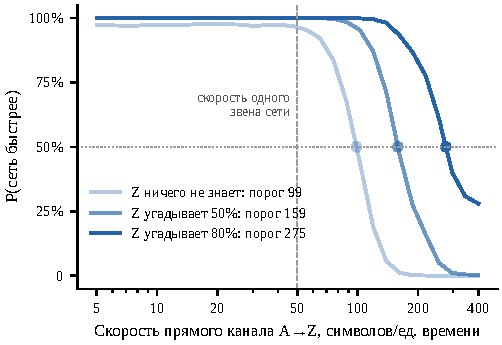
\includegraphics[width=\columnwidth]{figures/fig_sim.pdf}
\caption{Вероятность, что сеть восстановит сообщение раньше прямого канала. Знания $Z$ сдвигают порог почти втрое: с 99 до 275 символов за единицу времени.}
\label{fig:sim}
\end{figure}

Пока прямой канал не быстрее звена сети, сеть выигрывает в 97–100\% прогонов (рис.~\ref{fig:sim}).

Допустимая ошибка без кодирования не заменяет избыточность, но повышает устойчивость к искажениям (табл.~\ref{tab:corr}).

\begin{table}[t]
\centering\small
\caption{Вероятность выигрыша сети при прямом канале 40 символов за единицу времени.}
\label{tab:corr}
\begin{tabular}{@{}lccc@{}}
\toprule
Искажения & Точно & 80\% & 60\% \\
\midrule
0\% & 100\% & 100\% & 100\% \\
5\% & 88\% & 77\% & 98\% \\
10\% & 44\% & 43\% & 88\% \\
20\% & 3\% & 8\% & 43\% \\
30\% & 0\% & 1\% & 13\% \\
\bottomrule
\end{tabular}
\end{table}

\textbf{Повторение вместо кода.} Люди не кодируют слухи, а пересказывают. Каждый из 10 кусков пересказывают трое; с вероятностью $\rho$ кусок искажён уже у источника слуха. Подтверждение от двух источников убирает случайные искажения, но сильно замедляет и почти не защищает от общего источника (табл.~\ref{tab:gossip}).

\begin{table}[t]
\centering\small
\caption{Сарафан с повторением: нужно 80\% верного, медленный прямой канал.}
\label{tab:gossip}
\begin{tabular}{@{}cccc@{}}
\toprule
$\rho$ & \multicolumn{2}{c}{Сеть быстрее} & Ложь принята \\
 & верить первому & ждать двух & первому / двух \\
\midrule
0 & 90\% & 24\% & 8\% / 0\% \\
0,1 & 67\% & 14\% & 17\% / 10\% \\
0,3 & 19\% & 3\% & 36\% / 30\% \\
\bottomrule
\end{tabular}
\end{table}

\section{Пример: слухи о реструктуризации}

Совет директоров ($A$) утвердил реструктуризацию, официально её объявят через 14 дней. План в части отдела $Z$ описывается тремя параметрами: что будет с отделом (4 варианта), когда (12 месяцев), кто возглавит направление (8 кандидатов). Информация доходит до окружения $Z$ не раньше чем через 2 дня; примем $C=0{,}5$ бита в день — это допущение.
\[
C\,(T-1-d) = 0{,}5\cdot(14-1-2) = 5{,}5\ \text{бита}.
\]

\begin{center}\small
\begin{tabular}{@{}lccc@{}}
\toprule
Что нужно $Z$ & $|M|$ & $V(\varepsilon)$ & бит \\
\midrule
Всё, без контекста & 384 & 1 & 8,6 \\
Всё, с контекстом & 24 & 1 & 4,6 \\
«Под ударом или нет» & 24 & 12 & 1 \\
\bottomrule
\end{tabular}
\end{center}

Главное ($1$ бит) сеть доставляет к 4-му дню, за 10 дней до объявления; искажения в деталях не мешают, потому что входят в допустимую ошибку. Вывод устойчив по $C$ (табл.~\ref{tab:range}).

\begin{table}[t]
\centering\small
\caption{День, к которому сеть доставляет нужное ($d=2$, объявление на 14-й день; «—» — не успевает).}
\label{tab:range}
\begin{tabular}{@{}cccc@{}}
\toprule
$C$, бит/день & 8,6 бита & 4,6 бита & 1 бит \\
\midrule
0,1 & — & — & 12 \\
0,5 & — & 12 & 4 \\
2 & 7 & 5 & 3 \\
\bottomrule
\end{tabular}
\end{table}

\subsection{Как измерить $C$: обратная задача}

Теорему 1$'$ можно читать наоборот: если $Z$ верно восстановил главное к моменту $\tau$, то
\[
C \;\ge\; \frac{\log_2 N(\varepsilon)}{\tau-d}.
\]
\leanref{\lean{Exact.inverse_capacity}.}
Если опрос показал, что руководители отделов верно знали «под ударом или нет» к 4-му дню при $d=2$, то $C\ge 0{,}5$ бита в день. Процедура: взять прошлое решение с известными датами; сформулировать вопрос, от которого зависели решения сотрудников, и посчитать $\log_2 N(\varepsilon)$; установить $\tau$ и $d$ по опросу или переписке; повторить на нескольких событиях. Это нижняя оценка; ретроспективные опросы искажаются памятью, и учитывать нужно также тех, кто угадал неверно.

\section{Асимметричная информация}

Сколько раскрывает намёк, определяется не самим намёком, а тем, что уже знает получатель.

\begin{stmt}{Предложение 1 (контекст решает)}
Для подсказки $h=x+\mathit{key}$ в группе $G$:
\[
\begin{gathered}
\{x:\exists\,\mathit{key},\ x+\mathit{key}=h\}=G,\\
\{x: x+\mathit{key}=h\}=\{h-\mathit{key}\}.
\end{gathered}
\]
\end{stmt}
Одна и та же фраза даёт постороннему 0 бит, а знающему — всё сообщение.
\leanref{\lean{context_decides}.}

\begin{stmt}{Предложение 2 (мозаика, схема Шамира~\cite{shamir})}
Любые $k$ значений многочлена степени $<k$ определяют секрет $p(0)$; любые $k-1$ совместимы с каждым секретом ровно одним способом:
\[
\forall s'\ \exists!\,p:\ \deg p<k,\ p(0)=s',\ p(x_i)=v_i.
\]
\end{stmt}
\begin{proof}
Существование — интерполяция Лагранжа по $k$ точкам $0,x_1,\dots,x_{k-1}$; единственность — многочлены степени $<k$, совпадающие в $k$ точках, равны.
\end{proof}
\leanref{\lean{shamir_reconstruct}, \lean{shamir_private}.}

\begin{stmt}{Предложение 3 (риск утечки)}
Если $k$ посвящённых независимо проговариваются с вероятностью $q$ в день, то риск за $T$ дней
\[
\frac{kTq}{1+kTq}\le 1-(1-q)^{kT}\le kTq.
\]
\end{stmt}
\leanref{\lean{leak_le}, \lean{noLeak_mul_le}, \lean{safe_window}.}

\begin{stmt}{Предложение 3$'$ (круги вместо людей)}
Если посвящённые разбиты на независимые круги, круг $j$ проговаривается с вероятностью $p_j\le q$, а внутри круга утечки связаны как угодно, то
\[
1-\prod_j(1-p_j)^T \le T\sum_j p_j \le g\,T\,q,
\]
где $g$ — число кругов.
\end{stmt}
\begin{proof}
Неравенство Вейерштрасса $\prod(1-p_j)\ge1-\sum p_j$ и неравенство Бернулли.
\end{proof}
\leanref{\lean{Exact.weierstrass}, \lean{Exact.leak_clusters_le}, \lean{Exact.leak_clusters_uniform}.}

Риск определяется числом независимых кругов, а не числом людей (рис.~\ref{fig:leak}). Сократить число кругов вдвое так же полезно, как объявить вдвое раньше.

\begin{figure}[t]
\centering
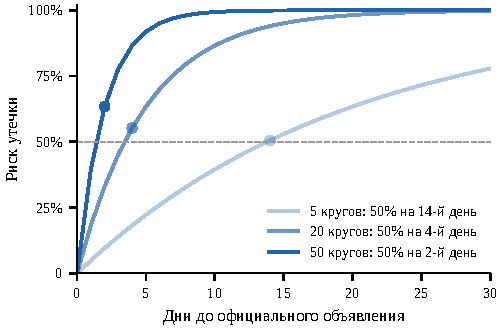
\includegraphics[width=\columnwidth]{figures/fig_leak.pdf}
\caption{Риск утечки при $q=1\%$ в день на круг: выше 50\% на 2-й день при 50 кругах и на 14-й при 5.}
\label{fig:leak}
\end{figure}

\section{Конфликт интересов}

Если у передающего есть свой интерес $b$, за один раунд честно проходит не больше $\log_2 N(b)$ бит. Модель~\cite{crawfordsobel}: отправитель знает $\theta\in[0,1]$ (равномерно), получатель хочет действие $a=\theta$, отправитель — $a=\theta+b$; потери квадратичные, слова не проверяются. В равновесии отправитель сообщает номер интервала $[a_i,a_{i+1}]$, получатель выбирает его середину $m_i$.

\begin{stmt}{Теорема 3}
При $b\ge0$ равновесие с $N$ интервалами существует тогда и только тогда, когда
\[
2N(N-1)\,b<1.
\]
\end{stmt}
\begin{proof}
($\Rightarrow$) Тип $\theta=a_{i+1}$ принадлежит обоим соседним интервалам, поэтому ему безразлично: $(m_i-a_{i+1}-b)^2=(m_{i+1}-a_{i+1}-b)^2$, откуда
\[
a_{i+1}+b=\tfrac{m_i+m_{i+1}}{2}\ \Rightarrow\ a_{i+2}-a_{i+1}=(a_{i+1}-a_i)+4b.
\]
По индукции $a_k=kg+2bk(k-1)$, где $g>0$ — длина первого интервала; при $k=N$: $2N(N-1)b=1-Ng<1$.
($\Leftarrow$) Положим $g=(1-2N(N-1)b)/N>0$ и построим границы по той же формуле; идеальное действие $\theta+b$ лежит между серединами соседних пар, поэтому отклоняться невыгодно.
\end{proof}
\leanref{\lean{IsEquilibrium.indiff}, \lean{crawford_sobel}, \lean{exists_equilibrium}, \lean{equilibrium_exists_iff}, \lean{no_info}.}

\begin{figure}[t]
\centering
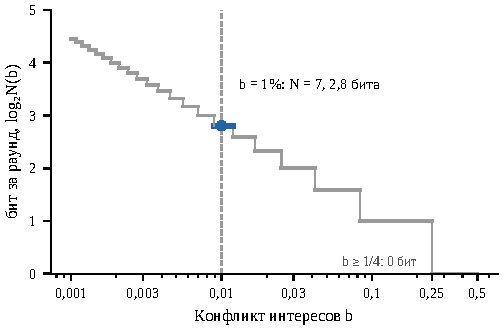
\includegraphics[width=\columnwidth]{figures/fig_cheap.pdf}
\caption{Максимум честно передаваемых бит $\log_2 N(b)$: при $b=1\%$ — 7 интервалов (2,8 бита), при $b\ge1/4$ — ноль.}
\label{fig:cheap}
\end{figure}

Следовательно, в слухах и переговорах пропускная способность $C$ из теоремы~1 измеряется в правдоподобных битах, а не в словах (рис.~\ref{fig:cheap}). Ограничение снимается, если информацию можно проверить, или при нескольких источниках с противоположными интересами~\cite{krishnamorgan}.

\section{Постепенное раскрытие}

Когда источник раскрывает решение по частям, порядок важнее скорости. К моменту $\tau$ официальные заявления оставили множество $M_\tau$, которое со временем только уменьшается.

\begin{stmt}{Теорема 4}
$Z$ может решить в момент $\tau$ тогда и только тогда, когда $M_\tau$ покрывается шарами ошибки в пределах бюджета слухов:
\[
\begin{gathered}
\tau_{\txt{слухи}}=\min\{\tau:\lceil\log_2N_\tau(\varepsilon)\rceil\le C(\tau-d)\},\\
\tau_{\txt{офиц}}=\min\{\tau:N_\tau(\varepsilon)=1\},
\end{gathered}
\]
опережение слухов равно $\tau_{\txt{офиц}}-\tau_{\txt{слухи}}$.
\end{stmt}
\leanref{\lean{Disclosure.decide_iff_covers}, \lean{decide_later}, \lean{fuller_policy_not_later}.}

Частичное заявление, не отвечающее на главный вопрос, уменьшает $N_\tau(\varepsilon)$ и тем самым \emph{помогает слухам}.

\begin{stmt}{Теорема 5 (порядок раскрытия)}
Если официальный канал за период отвечает на один вопрос «да/нет», а решение $Z$ зависит от $K$ классов, то при любом порядке нужно не меньше $\log_2K$ периодов, а порядок «сначала главное» укладывается в $\lceil\log_2K\rceil$.
\end{stmt}
\begin{proof}
Если ответы на $t$ вопросов определяют класс, класс — функция от вектора ответов, а векторов $2^t$. Порядок «сначала главное»: пронумеровать классы и спрашивать биты номера.
\end{proof}
\leanref{\lean{order_lower}, \lean{order_decision_first}, \lean{detail_first_slow}, \lean{decision_first_fast}.}

\begin{stmt}{Предложение 4 (молчание как сигнал)}
Если источник сообщает только о хороших темах и это правило известно $Z$, по сказанному однозначно восстанавливаются все $k$ тем: умолчание даёт до $k$ бит (эффект раскручивания~\cite{milgrom}).
\end{stmt}
\leanref{\lean{silence_reveals}.}

\begin{table*}[t]
\centering\small
\caption{Постепенное раскрытие: решение $Z$ зависит от 3 кусков из 10; официально — по куску каждые 5 единиц времени.}
\label{tab:disc}
\begin{tabular}{@{}lcccccc@{}}
\toprule
Политика & $\rho$ & Главное раскрыто & Опережение слухов & Решил раньше & Раньше и неверно \\
\midrule
Всё в конце & 0 & 51 & 39 & 89\% & 20\% \\
Сначала детали & 0 & 50 & 38 & 97\% & 22\% \\
Сначала главное & 0 & 15 & 5 & 89\% & 11\% \\
Всё в конце & 0,3 & 51 & 39 & 89\% & 65\% \\
Сначала детали & 0,3 & 50 & 38 & 97\% & 70\% \\
Сначала главное & 0,3 & 15 & 5 & 89\% & 49\% \\
\bottomrule
\end{tabular}
\end{table*}

\begin{table*}[t]
\centering\small
\caption{Преждевременные действия: 200 сотрудников, 8 отделов, 3 затронуты, ответ на 20-й день, заявления на 5-й день; 2000 прогонов.}
\label{tab:actions}
\begin{tabularx}{\textwidth}{@{}Xccc@{}}
\toprule
Что делает источник & Лишних действий & Доля незатронутых, кто действовал & Доля затронутых, кто успел \\
\midrule
Молчит до 20-го дня & 18,4 & 15\% & 37\% \\
Объявляет только дату ответа & 9,0 & 7\% & 17\% \\
Частично: «два отдела не затронуты» & 28,5 & 23\% & 58\% \\
Сначала главное: каждый отдел знает статус & 7,4 & 6\% & 100\% \\
\bottomrule
\end{tabularx}
\end{table*}

В симуляции (табл.~\ref{tab:disc}) порядок «сначала главное» сокращает опережение слухов с 38 до 5 единиц и почти вдвое — долю решений на неверных данных. «Сначала детали» даже помогает слухам: доля решений раньше ответа растёт с 89 до 97\%.

\begin{table*}[t]
\centering\small
\caption{Проверяемые предсказания.}
\label{tab:pred}
\begin{tabularx}{\textwidth}{@{}>{\raggedright\arraybackslash}p{0.27\textwidth}>{\raggedright\arraybackslash}p{0.14\textwidth}>{\raggedright\arraybackslash}X>{\raggedright\arraybackslash}X@{}}
\toprule
Предсказание & Основание & Как проверить & Что опровергнет \\
\midrule
1. Сотрудники с большим контекстом узнают главное раньше & Теорема 1$'$ & Опрос после объявления: когда узнали, что знали заранее & Нет связи между контекстом и моментом верного знания \\
2. Время до утечки обратно пропорционально числу независимых кругов & Предложение 3$'$ & Списки посвящённых, их группы, дата первого слуха & Время лучше объясняется числом людей \\
3. Чем сильнее конфликт интересов источника, тем грубее слух & Теорема 3 & Сравнить слухи из заинтересованных и незаинтересованных источников & Заинтересованные передают столь же точные детали \\
4. Частичное заявление без ответа на главный вопрос ускоряет слухи & Теорема 4 & Время до «все знают главное» с тизером и без & После тизера слухи о главном не появляются раньше \\
5. «Сначала главное» даёт меньше решений на неверных слухах & Теорема 5 & Сравнить объявления по порядку раскрытия & Порядок не влияет на долю ошибочных решений \\
6. Раннее закрытие главного вопроса снижает лишние действия & Предложение 5 & Доля действий, названных лишними, при раннем и позднем закрытии & Ранее закрытие не снижает эту долю \\
\bottomrule
\end{tabularx}
\end{table*}

\section{Следствие: преждевременные действия}

Пока официального ответа нет, люди действуют на том, что знают, и часть действий оказывается лишней. \emph{Гипотеза}: даже частичное раскрытие главных фактов сокращает действия, которые не были бы совершены при полной информации. Пример: менеджер не пошёл бы искать работу, если бы заранее знал ключевые детали анонса.

\begin{dfn}{Определения}
Лишнее действие совершено до официального ответа и не было бы совершено при полной информации; упущенное — наоборот. $Z$ действует, когда вероятность плохого исхода не меньше личного порога $\theta$.
\end{dfn}

\begin{stmt}{Предложение 5}
Пусть $U$ — те, кому главный вопрос не закрыт. При $\theta>0$
\[
\#\{\txt{лишние}\}\le\#\{i\in U: i\ \txt{не затронут}\},
\]
а при $U=\varnothing$ нет ни лишних, ни упущенных действий.
\end{stmt}
\leanref{\lean{Actions.regret_only_unresolved}, \lean{full_resolution}.}

\begin{table}[t]
\centering\small
\caption{8 отделов, 3 затронуты: лишние (Л) и упущенные (У) действия. Проверено в Lean.}
\label{tab:regret}
\setlength{\tabcolsep}{3.5pt}
\begin{tabular}{@{}lccc@{}}
\toprule
Что известно & Л, $\theta{=}30\%$ & Л, $\theta{=}50\%$ & У, $\theta{=}50\%$ \\
\midrule
Только слухи (3/8) & 5 & 0 & 3 \\
«Два отдела не затронуты» & 3 & \textbf{3} & 0 \\
Каждый знает статус & 0 & 0 & 0 \\
\bottomrule
\end{tabular}
\end{table}

Частичное раскрытие может дать обратный эффект (табл.~\ref{tab:regret}): при $\theta=50\%$ оно повышает тревогу у тех, кому вопрос не закрыт, и добавляет 3 лишних действия, зато упущенных становится 0.
\leanref{\lean{partial_can_increase_regret}, \lean{partial_can_decrease_regret}, \lean{partial_reduces_missed}.}

\begin{stmt}{Предложение 6 (ценность информации)}
Если раскрытие $c'$ подробнее $c$, то для любого правила $\pi$
\[
\min_{\pi'}\sum_x f(\pi'(c'(x)),x)\le\sum_x f(\pi(c(x)),x).
\]
\end{stmt}
\leanref{\lean{best_policy}, \lean{value_of_information}, \lean{refinement_helps}.}
Сумма лишних и упущенных действий не растёт; меняется их состав.

\begin{stmt}{Предложение 7 (объявленная дата)}
$Z$ действует сразу, если $(1-p)R<p\,c\,w$, где $w$ — ожидаемый срок ответа. Кто ждёт при сроке $w$, ждёт и при любом меньшем.
\end{stmt}
\leanref{\lean{shorter_wait_fewer_actions}.}



\textbf{Итог для гипотезы.} Гипотеза верна в уточнённой форме: раскрытие главного факта сокращает лишние действия тех, для кого оно полностью закрывает вопрос, и тем сильнее, чем раньше сделано (табл.~\ref{tab:actions}). Частичное раскрытие, оставляющее вопрос открытым, может увеличить их в полтора раза.

\textbf{Что делать источнику.}
\begin{enumerate}
\item Для каждой группы закрывать её главный вопрос целиком.
\item Сообщать, кого решение не касается, сразу для всех незатронутых.
\item Делать это как можно раньше.
\item Если ответа нет — объявить дату, когда он будет.
\item О тех, по кому решения нет, говорить явно: молчание прочитают как плохой знак.
\end{enumerate}

\section{Проверяемые предсказания}

Если предсказания не подтвердятся на данных, модель неверна, сколько бы теорем ей ни соответствовало. Для проверки достаточно 5–10 прошлых решений одной компании (табл.~\ref{tab:pred}).



\section{Формальная проверка в Lean 4}

Все теоремы статьи (их 91) записаны и доказаны в Lean~4.35.0 с Mathlib v4.35.0; пропущенных шагов (\lean{sorry}) нет; {\footnotesize\texttt{\#print axioms}} показывает только стандартные аксиомы \lean{propext}, \lean{Quot.sound} и \lean{Classical.choice}. Леммы о жадной раскраске и неравенство Вейерштрасса доказаны заново.

\begin{center}\small
\begin{tabular}{@{}lr@{}}
\toprule
Модуль & Теорем \\
\midrule
\lean{Sarafan.lean} & 32 \\
\lean{SarafanMosaic.lean} & 12 \\
\lean{SarafanCheapTalk.lean} & 11 \\
\lean{SarafanExact.lean} & 15 \\
\lean{SarafanDisclosure.lean} & 12 \\
\lean{SarafanActions.lean} & 9 \\
\bottomrule
\end{tabular}
\end{center}

Формулировка теоремы 1:
\begin{Verbatim}[fontsize=\scriptsize,frame=lines,framesep=2mm]
theorem rumour_general {M} [Fintype M]
  (dist : M → M → ℕ) (r V : ℕ)
  (hV : ∀ c, (univ.filter
     (fun x => dist c x ≤ r)).card ≤ V)
  (bits : ℕ → ℕ) (d C tDirect : ℕ)
  (hcap : ∀ τ, bits τ ≤ C * (τ - d))
  (hwin : ∃ τ < tDirect, ∃ enc dec,
     ∀ x, dist (dec (enc x)) x ≤ r) :
  Fintype.card M
    ≤ 2 ^ (C * (tDirect - 1 - d)) * V
\end{Verbatim}

Lean гарантирует, что выводы следуют из предположений. Сами предположения — вопрос к реальности: сеть описывается числом $C$ после задержки $d$; знания $Z$ — множеством совместимых сообщений; круги посвящённых независимы; в модели Кроуфорда–Собела середина интервала задана, а не выведена.

\section{Ограничения и открытые вопросы}

\begin{itemize}
\item \textbf{Асимптотическая достаточность} для длинных сообщений следует из теорем Шеннона, Слепяна–Вулфа и Вайнера–Зива~\cite{shannon,slepianwolf,wynerziv}, но в Lean не формализована. Для однократной передачи точный ответ дают теоремы 1$'$ и 2.
\item \textbf{Худший случай вместо вероятностей.} Версия «с вероятностью не менее $1-\delta$» потребует теории меры.
\item \textbf{Не формализованы} модель Кайла, парадокс Гроссмана–Стиглица и теорема Кондорсе в вероятностной форме.
\item \textbf{Эмпирика.} Утверждения о реальных организациях проверяются данными, а не доказательствами; теорема говорит лишь, при каких условиях эффект возможен.
\item \textbf{Числа в примерах заданы, а не измерены.} Обратная задача даёт способ измерения, но только нижнюю оценку $C$, и на реальных данных она ещё не применялась.
\end{itemize}

Остающиеся предположения стоит ослабить следующими: середину интервала в модели Кроуфорда–Собела вывести, а не постулировать; допустить связь между кругами посвящённых; описывать $C$ как функцию времени и темы.

\begin{thebibliography}{99}
\small
\setlength{\itemsep}{1pt}
\bibitem{ahlswede} R.~Ahlswede, N.~Cai, S.-Y.~R.~Li, R.~W.~Yeung. Network information flow. \textit{IEEE Trans. Inf. Theory}, 46(4), 2000.
\bibitem{shannon} C.~E.~Shannon. Coding theorems for a discrete source with a fidelity criterion. \textit{IRE Nat. Conv. Record}, 1959.
\bibitem{slepianwolf} D.~Slepian, J.~K.~Wolf. Noiseless coding of correlated information sources. \textit{IEEE Trans. Inf. Theory}, 19(4), 1973.
\bibitem{wynerziv} A.~D.~Wyner, J.~Ziv. The rate-distortion function for source coding with side information at the decoder. \textit{IEEE Trans. Inf. Theory}, 22(1), 1976.
\bibitem{witsenhausen} H.~S.~Witsenhausen. The zero-error side information problem and chromatic numbers. \textit{IEEE Trans. Inf. Theory}, 22(5), 1976.
\bibitem{crawfordsobel} V.~P.~Crawford, J.~Sobel. Strategic information transmission. \textit{Econometrica}, 50(6), 1982.
\bibitem{shamir} A.~Shamir. How to share a secret. \textit{Communications of the ACM}, 22(11), 1979.
\bibitem{krishnamorgan} V.~Krishna, J.~Morgan. A model of expertise. \textit{Quarterly Journal of Economics}, 116(2), 2001.
\bibitem{shibutani} T.~Shibutani. \textit{Improvised News: A Sociological Study of Rumor}. Bobbs-Merrill, 1966.
\bibitem{difonzo} N.~DiFonzo, P.~Bordia. \textit{Rumor Psychology: Social and Organizational Approaches}. APA, 2007.
\bibitem{karp} R.~M.~Karp, C.~Schindelhauer, S.~Shenker, B.~Vöcking. Randomized rumor spreading. \textit{FOCS}, 2000.
\bibitem{affeldt} R.~Affeldt, M.~Hagiwara, J.~Sénizergues. Formalization of Shannon's theorems. \textit{J. Automated Reasoning}, 53(1), 2014.
\bibitem{milgrom} P.~Milgrom. Good news and bad news: representation theorems and applications. \textit{Bell Journal of Economics}, 12(2), 1981.
\end{thebibliography}

\end{document}
